%============================================================================
% tento soubor pouzijte jako zaklad
% (c) 2008 Michal Bidlo
% E-mail: bidlom AT fit vutbr cz
%============================================================================
% kodovaní: utf-8 (zmena prikazem iconv, recode nebo cstocs)
%----------------------------------------------------------------------------
% zpracování: make, make pdf, make desky, make clean
% připomínky posílejte na e-mail: bidlom AT fit.vutbr.cz
% vim: set syntax=tex encoding=utf8:
%============================================================================

%nezpracovava se pomoci pdflatex
\let\pdfoutput\undefined

%\documentclass[cover,english]{fitthesis} % odevzdani do wisu - odkazy, na ktere se da klikat
%\documentclass[english, cover]{fitthesis} % odevzdani do wisu - odkazy, na ktere se da klikat
\documentclass[cover,print]{fitthesis} % pro tisk - na odkazy se neda klikat
%\documentclass[english,print]{fitthesis} % pro tisk - na odkazy se neda klikat
%      \documentclass[english]{fitthesis}
% * Je-li prace psana v anglickem jazyce, je zapotrebi u tridy pouzit 
%   parametr english nasledovne:
%      \documentclass[english]{fitthesis}
% * Neprejete-li si vysazet na prvni strane dokumentu desky, zruste 
%   parametr cover

% zde zvolime kodovani, ve kterem je napsan text prace
% "latin2" pro iso8859-2 nebo "cp1250" pro windows-1250, "utf8" pro "utf-8"
%\usepackage{ucs}
\usepackage[utf8]{inputenc}
\usepackage[T1, IL2]{fontenc}
\usepackage{url}
\DeclareUrlCommand\url{\def\UrlLeft{<}\def\UrlRight{>} \urlstyle{tt}}

%zde muzeme vlozit vlastni balicky

\usepackage{amsthm}
\usepackage{amsmath}
\usepackage{mdwlist}

\usepackage[bf]{caption2}

%\theoremstyle{definition}
%\newtheorem{Def}{Definice}[section]
%\newtheorem{Alg}{Algoritmus}
%\newtheorem{Example}{Příklad}[section]
%\newtheorem{Veta}{Věta}

%\newcommand{\nt}[1]{$<$\textit{#1}$>$}
\newcommand{\N}[1]{\textit{#1}}
\newcommand{\T}[1]{\texttt{#1}}

% =======================================================================
% balíček "hyperref" vytváří klikací odkazy v pdf, pokud tedy použijeme pdflatex
% problém je, že balíček hyperref musí být uveden jako poslední, takže nemůže
% být v šabloně
\ifWis
\ifx\pdfoutput\undefined % nejedeme pod pdflatexem
\else
  \usepackage{color}
  \usepackage[unicode,colorlinks,hyperindex,plainpages=false,pdftex]{hyperref}
  \definecolor{links}{rgb}{0.4,0.5,0}
  \definecolor{anchors}{rgb}{1,0,0}
  \def\AnchorColor{anchors}
  \def\LinkColor{links}
  \def\pdfBorderAttrs{/Border [0 0 0] }  % bez okrajů kolem odkazů
  \pdfcompresslevel=9
\fi
\fi

%Informace o praci/projektu
%---------------------------------------------------------------------------
\projectinfo{
  %Prace
  project=SP,            %typ prace BP/SP/DP/DR
  year=2016,             %rok
  date=\today,           %datum odevzdani
  %Nazev prace
  title.cs={Optimalizace bajtkódu Javy s~ohledem na~jeho velikost},  %nazev prace v cestine
  title.en={Java Bytecode Size Optimization}, %nazev prace v anglictine
  %Autor
  author={Vendula Poncová},   %jmeno prijmeni autora
  author.title.p=Bc., %titul pred jmenem (nepovinne)
  %author.title.a=PhD, %titul za jmenem (nepovinne)
  %Ustav
  department=UITS, % doplnte prislusnou zkratku: UPSY/UIFS/UITS/UPGM
  %Skolitel
  supervisor=Radek Kočí, %jmeno prijmeni skolitele
  supervisor.title.p=Ing.,   %titul pred jmenem (nepovinne)
  supervisor.title.a={Ph.D.},    %titul za jmenem (nepovinne)
  %Klicova slova, abstrakty, prohlaseni a podekovani je mozne definovat 
  %bud pomoci nasledujicich parametru nebo pomoci vyhrazenych maker (viz dale)
  %===========================================================================
  %Klicova slova
  keywords.cs={Klíčová slova v českém jazyce.}, %klicova slova v ceskem jazyce
  keywords.en={Klíčová slova v anglickém jazyce.}, %klicova slova v anglickem jazyce
  %Abstract
  abstract.cs={Výtah (abstrakt) práce v českém jazyce.}, % abstrakt v ceskem jazyce
  abstract.en={Výtah (abstrakt) práce v anglickém jazyce.}, % abstrakt v anglickem jazyce
  %Prohlaseni
  declaration={Prohlašuji, že jsem tuto semestrální práci vypracovala samostatně pod vedením pana Ing. Radka Kočího, Ph.D. a pana Ing. Pavla Tišnovského, Ph.D. Uvedla jsem všechny literální prameny a publikace, ze kterých jsem čerpala.},
  %Podekovani (nepovinne)
  %acknowledgment={Zde je možné uvést poděkování vedoucímu práce a těm, kteří poskytli odbornou pomoc.} % nepovinne
}

%Abstrakt (cesky, anglicky)
%\abstract[cs]{Do tohoto odstavce bude zapsán výtah (abstrakt) práce v českém jazyce.}
%\abstract[en]{Do tohoto odstavce bude zapsán výtah (abstrakt) práce v anglickém jazyce.}

%Klicova slova (cesky, anglicky)
%\keywords[cs]{Sem budou zapsána jednotlivá klíčová slova v českém jazyce, oddělená čárkami.}
%\keywords[en]{Sem budou zapsána jednotlivá klíčová slova v anglickém jazyce, oddělená čárkami.}

%Prohlaseni
%\declaration{Prohlašuji, že jsem tuto bakalářskou práci vypracoval samostatně pod vedením pana X...
%Další informace mi poskytli...
%Uvedl jsem všechny literární prameny a publikace, ze kterých jsem čerpal.}

%Podekovani (nepovinne)
%\acknowledgment{V této sekci je možno uvést poděkování vedoucímu práce a těm, kteří poskytli odbornou pomoc
%(externí zadavatel, konzultant, apod.).}

\begin{document}
  % Vysazeni titulnich stran
  % ----------------------------------------------
  \maketitle
  % Obsah
  % ----------------------------------------------
  \tableofcontents
  
  % Seznam obrazku a tabulek (pokud prace obsahuje velke mnozstvi obrazku, tak se to hodi)
  % \listoffigures
  % \listoftables 

  % Text prace
  % ----------------------------------------------
  %=========================================================================

%%%%%%%%%%%%%%%%%%%%%%%%%%%%%%%%%%%%%%%%%%%%%%%%%%%%%%%%%%%%%%%%%%%%%%%%%%
\chapter{Úvod}\label{Introduction}

% Úvod do tématu. 

Kód programu je obvykle optimalizován s~cílem minimalizovat dobu běhu programu, ale hlavním požadavkem může být i kratší kód či efektivnější práce s~dostupnými prostředky, jak uvádí Aho \cite{}. Zatímco optimalizace rychlosti je u~jazyka Java dobře zpracovaným tématem \cite{}, optimalizace velikosti kódu se řeší především v~souvislosti s~vestavěnými systémy \cite{} a obfuskací \cite{}. Ve vestavěných systémech se však používají specializované edice Javy a obfuskace kódu vede k~modifikaci struktury programu. Kratší kód přitom zabírá méně paměti, rychleji se přenáší po síti a může vést i k~rychlejšímu běhu programu. Cílem této práce je proto studium bajtkódu Javy SE z~hlediska jeho velikosti a návrh metod pro optimalizaci velikosti bajtkódu. Výstupem práce jsou nástroje \texttt{jbyca} a \texttt{jbyco} pro analýzu a optimalizaci bajtkódu.

V~kapitole \ref{} se věnuji obecné speficikaci bajtkódu Javy. Popisuji virtuální stroj Java Virtual Machine, způsob, jakým je bajtkód interpretován, a zabývám se formátem, v~jakém je bajtkód uložen v~instrukčních souborech. V~kapitole \ref{Tools} uvádím stručný popis existujících nástrojů pro manipulaci s~bajtkódem a shrnuji jejich výhody a nevýhody. Konkrétně zmiňuji BCEL, ASM a Javassist. Tyto nástroje jsem využila při návrhu a implementaci nástroje \texttt{jbyca} pro analýzu bajtkódu popsaného v~kapitole \ref{}. Nástroj jsem aplikovala na vybraný vzorek dat a získané výstupy zpracovala a vyhodnotila v~kapitole \ref{}. Na základě výsledků jsem navrhla metody pro optimalizaci velikosti a implementovala je v~nástroji \texttt{jbyco}, kterému je věnovaná kapitola \ref{}. Nakonec jsem s užitím tohoto nástroje optimalizovala vzorová data a vyhodnotila účinky optimalizačních metod.


%=========================================================================


%%%%%%%%%%%%%%%%%%%%%%%%%%%%%%%%%%%%%%%%%%%%%%%%%%%%%%%%%%%%%%%%%%%%%%%%%%
\chapter{Java Virtual Machine}

Architektura Javy se skládá z programovacího jazyka Java, formátu instrukčního souboru, aplikačního programového rozhraní Java Application Programming Interface (Java API) a virtuálního stroje Java Virtual Machine (JVM) (). Pro psaní zdrojových kódů a jejich spouštění je zapotřebí všech těchto částí.
Zdrojový kód zapsaný v programovacím jazyce Java je uložený v souboru s příponou \texttt{.java} (dále \texttt{java} soubor). Tento kód je při kompilaci převeden na mezikód, tzv. bajtkód, a uložen v souborech s příponou \texttt{.class} (dále \texttt{class} soubory). Bajtkód lze spustit pomocí virtuálního stroje, který má přístup k Java API. O tomto stroji lze hovořit z hlediska abstraktní specifikace nebo konkrétní implementace (). Konkrétní implementace je závislá na daném systému a hardwaru, ale jednotná interpretace \texttt{class} souborů napříč platformami je zajištěna dodržením specifikace a platformově nezávislým formátem \texttt{class} souborů. Vzhledem k zaměření práce se v této kapitole zabývám abstraktní specifikací JVM dle dokumentu (). 

\section{Datové typy a hodnoty}

Primitivní datové typy a hodnoty podporované JVM jsou znázorněné na diagramu (). Celá čísla jsou reprezentovaná typy \texttt{byte} o délce 8 bitů, \texttt{short} o délce 16 bitů, \texttt{int} o délce 32 bitů nebo \texttt{long} o délce 64 bitů. Pro čísla s plovoucí čárkou jsou definovány typy \texttt{float} o 32 bitech a \texttt{double} o 64 bitech. Typ \texttt{boolean} reprezentuje pravdivostní hodnoty pravda a nepravda. Typ \texttt{returnAddress} reprezentuje ukazatel na instrukci v instrukčním souboru.

Znaky a řetězce jsou v Javě kódované podle standardu Unicode v kódování UTF-16, kde jeden znak je kódovaný jednou nebo dvěmi kódovými jednotkami. Kódovou jednotku reprezentuje typ \texttt{char}. Jedná se o 16-bitové nezáporné číslo. Řetězec je pak reprezentovaný pomocí pole hodnot typu \texttt{char}. V instrukčním souboru jsou řetězcové konstanty kódované v modifikovaném kódování UTF-8. 

Typ \texttt{reference} označuje referenční datový typ. Typ reprezentuje referenci na dynamicky vytvořený objekt. Podle toho, zda objekt je instancí třídy, pole nebo instancí třídy či pole, které implementují nějaké rozhraní, rozlišujeme typ reference. Hodnotou typu \texttt{reference} může být též speciální hodnota \texttt{null}, která reprezentuje referenci na žádný objekt. S objekty lze manipulovat výhradně skrze reference.


% TODO vylepšit, ošklivé

\begin{figure}[!h]
\centering

\begin{tikzpicture}[level distance=1.6in,sibling distance=.1in,scale=.6]
\tikzset{
  %edge from parent/.style= {thick, draw},
  every tree node/.style={draw,minimum width=.7in,text width=1in, align=center}, 
  edge from parent fork right,
  grow'=right,
}

\Tree
[.{datové typy}
[.{primitivní datové typy} 
  [.{numerické datové typy} 
    [.{celočíselné}
      [{\texttt{byte}} ]
      [{\texttt{short}} ]
      [{\texttt{int}} ]
      [{\texttt{long}} ]
      [{\texttt{char}} ]
    ] 
    [.{s plovoucí čárkou}
      [{\texttt{float}} ]
      [{\texttt{double}} ]
    ]
  ] 
  [.{logický datový typ}
      [{\texttt{boolean}} ]
  ] 
  [{\texttt{returnAddress}}]
]]
[.{referenční datový typ} [{\texttt{reference}} ]]
]

\end{tikzpicture}

\caption{Datové typy a hodnoty podporované JVM.}\label{figTypes}
\end{figure}



Instrukční sada JVM je omezená a nenabízí u všech instrukcí podporu pro všechny datové typy. Celá čísla jsou primárně reprezentovaná datovými typy \texttt{int} a \texttt{long} a případně přetypovaná na jeden z typů \texttt{byte}, \texttt{short} či \texttt{char}. Pro datový typ \texttt{boolean} existuje jen podpora pro přetypování a pro vytvoření pole hodnot typu \texttt{boolean}. Pro výpočet logických výrazů se používá typ \texttt{int} s hodnotami 0 a 1.


\section{Paměťové oblasti}

JVM pracuje s několika typy paměťových oblastí. Velikosti těchto oblastí mohou být pevně dané, nebo se mohou měnit dynamicky podle potřeby. Při spuštění JVM vzniká halda a oblast metod. Halda je paměť určená pro alokaci instancí tříd a polí. Alokovanou paměť nelze dealokovat explicitně. Haldu automaticky spravuje tzv. \textit{garbage collector}. Oblast metod slouží k ukládání kompilovaného kódu. Pro každou načtenou třídu se do této paměti ukládají struktury definující tuto třídu. Jednou z těchto struktur je tzv. \textit{run-time constant pool}. Jedná se o tabulku konstant z \texttt{class} souboru, kde jsou symbolické reference na třídy, metody a členské proměnné nahrazeny konkrétními referencemi. Více se o tabulce konstant zmiňuje kapitola (). Každá aplikace je spuštěna v samostaném vlákně a při běhu mohou vznikat a zanikat i další vlákna. Všechna taková vlákna sdílí přístup k haldě a oblasti metod. Navíc má každé vlákno k dispozici vlastní \texttt{pc} register a zásobník rámců. V \texttt{pc} registru je ucháván ukazatel na aktuálně vykonávanou instrukci, není-li aktuálně vykonávaná metoda nativní. Zásobník rámců uchovává data zavolaných metod. Při každém volání metody je vytvořen nový rámec. Rámec má vlastní pole lokálních proměnných a operační zásobník. V poli lokálních proměnných se uchovávají hodnoty parametrů a lokálních proměnných. Hodnoty lze vkládat na operační zásobník, provádět nad nimi výpočty a ukládat zpět do pole lokálních proměnných. Operační zásobník slouží k předávání operandů instrukcím a k uchovávání mezivýsledků. Podílí se také na předávání parametrů a návratových hodnot.

Před voláním metody je třeba neprve vložit parametry na operační zásobník aktuálního rámce. Zavoláním metody se vytvoří nový rámec a umístí se na vrchol zásobníku rámců. Parametry se následně přesunou z operačního zásobníku předchozího rámce do pole lokálních proměnných nového rámce. Registr \texttt{pc} se nastaví na první instrukci volané metody a začnou se vykonávat jednotlivé instrukce. Při návratu z metody je návratová hodnota umístěna na vrcholu operačního zásobníku, vrací-li metoda nějakou hodnotu. Tato hodnota je přesunuta na operační zásobník předcházejícího rámce a aktuální rámec je ze zásobníku rámců odstraněn. Dojde k obnovení stavu volající metody. Registr \texttt{pc} je nastaven na index instrukce, která bezprostředně následuje za instrukcí volajícící metodu. Pokud je metoda ukončena vyvoláním nezachycené výjimky, pak k předání hodnoty nedochází. Aktuální rámec je odstraněn a výjimka je znovu vyvolaná ve volající metodě. Zpracování výjimek je více vysvětleno v kapitole ().

Nejmenší jednotka, se kterou pracuje operační zásobník, je 32-bitová hodnota. Hodnoty většiny datových typů lze vyjádřit pomocí jedné jednotky, ale hodnoty typů \texttt{long} a \texttt{double} je třeba reprezentovat dvěmi jednotkami. S takovou dvojicí je třeba vždy manipulovat jako s celkem. Datový typ hodnoty na zásobníku je daný instrukcí, která ho tam vložila, a na hodnotu nelze nahlížet jinak. Hloubka operačního zásobníku je určená počtem jednotek na zásobníku. Proto se o jednotce dále zmiňuji jako o jednotce hloubky zásobníku.

Lokální proměnná v poli lokálních proměnných je 32-bitová hodnota. Proměnnou lze adresovat pomocí indexu do pole, kde pole je indexováno od nuly. Lokální proměnná může být typu \texttt{byte}, \texttt{short}, \texttt{int}, \texttt{char}, \texttt{float}, \texttt{boolean}, \texttt{reference} nebo \texttt{returnAddress}. Hodnoty typu \texttt{long} a \texttt{double} jsou uchovávané pomocí dvojice lokálních proměnných. V tom případě k adresaci slouží nižší z indexů a na větší index se nesmí přistupovat. 

\section{Kontrola instrukčního souboru}

Při načítání \texttt{class} souboru je ověřeno správné formátování tak, jak je popsáno v kapitole (). Jsou zkontrolovány první čtyři bajty souboru, předdefinované atributy musí být správné délky, názvy a typy tříd, rozhraní, metod a proměných musí být validní, indexy do tabulky konstant musí adresovat správný typ položky. Dále jsou kladena jistá omezení na kód metod. Mimo jiné, argumenty instrukcí musí mít správný typ a musí být správného počtu, integrita hodnot typu \texttt{long} a \texttt{double} nemůže být nikdy narušena, z hodnotě lokální proměnné se nesmí přistupovat před inicializací proměnné, nesmí dojít k načtení hodnoty z prázdného zásobníku, všechny metody musí byt ukončené \texttt{return} instrukcí. Verifikace těchto omezení se provádí pomocí typové kontroly nebo typové inference. Díky tomu se kontroly omezení nemusí provádět za běhu.


%=========================================================================

%%%%%%%%%%%%%%%%%%%%%%%%%%%%%%%%%%%%%%%%%%%%%%%%%%%%%%%%%%%%%%%%%%%%%%%%%%
\chapter{Formát instrukčního souboru}

% TODO
% * dopsat info u položek
% * definovat byte
% * nastudovat instrukce
% * ověřit velikosti "sdílených" nonterminálů !!!

Při kompilaci \texttt{java} souboru překladač pro každou definovanou třídu a rozhraní vytvoří jeden soubor s příponou \texttt{.class} (dále \texttt{class} soubor). Tento soubor obsahuje binární reprezentaci kompilovaného mezikódu, který lze interpretovat prostřednictvím JVM. V této kapitole popisuji formát \texttt{class} souboru dle specifikace ve verzi Java SE 8 Edition(X).

Pro popis formátu jsem zvolila rozšířenou Backus-Naurovu formu (?), která umožňuje zapsat syntaxi formálního jazyka pomocí pravidel a terminálních a nonterminálních symbolů. Nonterminální symboly jsou definovány pomocí definujícího symbolu \texttt{:=}, symbolu pro konkatenaci \texttt{,}, symbolu pro alternaci \texttt{$\mathtt{|}$}, symbolů pro nula a více opakování \texttt{\{\}}, ukončujícího symbolu \texttt{;} a pomocí graficky odlišených \T{terminálních} a \N{nonterminálních} symbolů.

\section{Základní struktura}

% Jaká je základní struktura class souboru?

Položky \texttt{class} souboru tvoří posloupnost osmibitových bajtů. Základní stavební jednotkou je tedy bajt, který je v pravidlech reprezentovaný symbolem \N{B}. Symbol $\langle n \rangle$\N{B}, kde $\langle n \rangle \in \{2,3,\dots\}$, reprezentuje $n$ bajtů. Terminály jsou hexadecimální reprezentací posloupnosti bajtů s prefixem \texttt{0x}. 

Základní struktura souboru je popsaná pravidlem pro symbol \N{classfile}. Soubor obsahuje informace o jeho typu a verzi (\N{version}), disponuje tabulkou všech konstant, které se v souboru vyskytují (\N{constants}), nese informace o třídě, kterou reprezentuje, případně rozhraní (\N{class}), obsahuje seznam rozhraní, které reprezentovaná třída implementuje, případně rozhraní rozšiřuje  (\N{interface\_list}), seznam členských proměnných třídy (\N{field\_list}), seznam metod (\N{method\_list}) a seznam atributů (\N{attribute\_list}). 

\begin{figure}[h!]
  \begin{tabular}{r c l}
  \N{classfile} &:=& \N{version}, \N{constants}, \N{class}, \N{interface\_list}, \N{field\_list}, \N{method\_list}, \N{attribute\_list};
  \end{tabular}
\end{figure}

Typ souboru je definován prvními čtyřmi bajty, které jsou popsané symbolem \N{magic\_number}. Verze souboru je tvořena hodnotou $M$ symbolu \N{major\_version} a hodnotou $m$ symbolu \N{minor\_version} jako $M.m$.

\begin{figure} [h!]
  \begin{tabular}{r c l}
  \N{version} &:=& \N{magic\_number}, \N{minor\_version}, \N{major\_version};\\
  \N{magic\_number} &:=& \T{0xCAFEBABE};\\
  \N{minor\_version} &:=& \N{2B};\\
  \N{major\_version} &:=& \N{2B};\\
  \end{tabular}
\end{figure}

\section{Konstanty}

% Popis struktury constant\_pool. Jakým způsobem jsou ukládané konstanty? Jak jsou reprezentované různé typy?
% Jednotlivé typy konstant lze nejspíš popsat jen slovně.
% TODO
% * zmínit run-time constant pool, kdy se symbolické reference nahrazují konkrétními referencemi

Tabulka konstant obsahuje některé číselné konstanty, všechny řetězce a symbolické informace o všech třídách, rozhraních, metodách a členských proměnných, které se v souboru, instrukcích i atributech vyskytují. Tato tabulka se nazývá \textit{constant pool} a slouží v podstatě jako databáze dat, do které se pomocí indexů odkazují další položky souboru. 

Struktura tabulky konstant je popsána pravidlem pro \N{constants}. Symbol \N{constant\_pool\_count} reprezentuje hodnotu $1 + n$, kde $n$ je počet položek v tabulce konstant. Položky tabulky jsou indexované od jedné. Nultý index je vyhrazen pro odkaz na žádnou z položek. Samotná tabulka je reprezentovaná symbolem \N{constant\_pool}.

\begin{figure} [h!]

  \begin{tabular}{r c l}
  \N{constants} &:=& \N{constant\_pool\_count}, \N{constant\_pool}; \\
  \N{constant\_pool\_count} &:=& \N{2B}; \\
  \N{constant\_pool} &:=& \{
          \N{constant\_integer} \\
  &&  $|$ \N{constant\_float} \\
  &&  $|$ \N{constant\_long} \\
  &&  $|$ \N{constant\_double} \\ 
  &&  $|$ \N{constant\_utf8} \\
  &&  $|$ \N{constant\_string} \\ 
  &&  $|$ \N{constant\_nameAndType} \\ 
  &&  $|$ \N{constant\_class} \\
  &&  $|$ \N{constant\_fieldref} \\
  &&  $|$ \N{constant\_methodref} \\
  &&  $|$ \N{constant\_interfaceMethodref} \\
  &&  $|$ \N{constant\_methodHandle} \\ 
  &&  $|$ \N{constant\_methodType} \\
  &&  $|$ \N{constant\_invokeDynamic} \\ 
  &&  \}; \\
  \end{tabular}
\end{figure}

Každá položka tabulky je tvořena označením typu a posloupností bajtů s informacemi o položce. Položky mohou mít různou velikost v závislosti na svém typu a obsahu. Stejným způsobem jsou definovány všechny tabulky v \texttt{class} souboru. Jestliže se jedná o pole, pak prvky pole jsou stejného typu, a proto označení typu v prvcích chybí.

 Číselné konstanty jsou reprezentované symboly \N{constant\_integer}, \N{constant\_float}, \N{constant\_long} a \N{constant\_double} a skládají se jen z typu a číselné hodnoty. 
Symbol \N{constant\_utf8} reprezentuje řetězec v upraveném kódování \texttt{UTF-8} a skládá se z typu, délky pole bajtů a pole bajtů nesoucích reprezentaci řetězce. Znaky řetězce mohou být vhledem ke kódování tvořeny různými počty bajtů. 
Symbol \N{constant\_string} je reprezentací řetězcové konstanty a kromě typu obsahuje index do tabulky konstant na položku \N{constant\_utf8}. 
Třídy a rozhraní jsou reprezentované položkami \N{constant\_class} s odkazy na jejich název (\N{constant\_utf8}). 
Entity jako členské proměnné, metody třídy a metody rozhraní jsou reprezentované položkami \N{constant\_fieldref}, \N{constant\_methodref} a \N{constant\_interfaceMethodref} obsahujícími odkaz na třídu, případně rozhraní, dané entity (\N{constant\_class}), a odkaz na položku se jménem a typem této entity (\N{constant\_nameAndType}). 
Jméno a typ v položce \N{constant\_nameAndType} jsou odkazy na řetězce (\N{constant\_utf8}). 
Položky \N{constant\_methodHandle}, \N{constant\_methodType} a \N{constant\_invokeDynamic} souvisí s podporou dynamických jazyků.

\section{Třída}

\begin{tabular}{r c l}
\N{class} &:=& \N{access\_flags}, \N{this\_class}, \N{super\_class};\\
\N{access\_flags} &:=& \N{2B}; \\
\N{this\_class} &:=& \N{class\_ref};\\
\N{super\_class} &:=& \N{class\_ref};\\
\N{class\_ref} &:=& \N{constant\_pool\_index}; \\
\N{constant\_pool\_index} &:=& \N{2B}; \\
\end{tabular}
\medskip

\section{Členské proměnné}

% Popis struktury field\_info. Jakým způsobem jsou uložené členské proměnné?

\begin{tabular}{r c l}
\N{field\_list} &:=& \N{fields\_count}, \N{fields};\\
\N{fields} &:=& \{ \N{field\_info} \};\\
\N{field\_info} &:=& \N{access\_flags}, \N{name\_ref}, \N{descriptor\_ref}, \N{attribute\_list};\\
\N{fields\_count} &:=& \N{2B};\\
\N{name\_ref} &:=& \N{utf8\_ref};\\
\N{descriptor\_ref} &:=& \N{utf8\_ref};\\
\N{utf8\_ref} &:=& \N{constant\_pool\_index}; \\
\end{tabular}
\medskip

\section{Metody}

% Popis struktury method\_info. Jakým způsobem jsou uložené metody? Kde jsou uloženy instrukce?

\begin{tabular}{r c l}
\N{interface\_list} &:=& \N{interface\_count}, \N{interfaces};\\
\N{interfaces} &:=& \{ \N{class\_ref} \};\\
\N{interface\_count} &:=& \N{2B};\\
\end{tabular}
\medskip

\begin{tabular}{r c l}
\N{method\_list} &:=& \N{methods\_count}, \N{methods};\\
\N{methods} &:=& \{ \N{method\_info} \};\\
\N{method\_info} &:=& \N{access\_flags}, \N{name\_ref}, \N{descriptor\_ref}, \N{attribute\_list};\\
\N{methods\_count} &:=& \N{2B};\\
\end{tabular}
\medskip

\medskip

\begin{tabular}{r c l}
\N{code\_info} &:=& \N{max\_stack}, \N{max\_locals}, \N{code\_list}, \N{exception\_list}, \N{attribute\_list}; \\ 
\N{code\_list} &:=& \N{code\_length}, \N{code} ; \\ 
\N{code} &:=& \{ \N{B} \}; \\ 
\N{max\_stack} &:=& \N{2B}; \\ 
\N{max\_locals} &:=& \N{4B}; \\ 
\N{code\_length} &:=& \N{4B} ; \\ 


\end{tabular}
\medskip


\begin{tabular}{r c l}
\N{exception\_list} &:=& \N{exception\_table\_length}, \N{exception\_table} ; \\ 
\N{exception\_table} &:=& \{ \N{\N{start\_pc}, \N{end\_pc}, \N{handler\_pc}, \N{catch\_type}} \}; \\ 
\N{start\_pc} &:=& \N{code\_index}; \\ 
\N{end\_pc} &:=& \N{code\_index}; \\ 
\N{handler\_pc} &:=& \N{code\_index}; \\ 
\N{catch\_pc} &:=& \N{class\_ref}; \\ 
\N{exception\_table\_length} &:=& \N{2B}; \\ 
\N{code\_index} &:=& \N{2B}; \\

\end{tabular}
\medskip

\section{Instrukce}

% Přehled instrukcí a krátké příklady bajkódu.

\section{Atributy}

% Základní přehled atributů, jen ty podstatné, neboť jich je mnoho.

\begin{tabular}{r c l}
\N{attribute\_list} &:=& \N{attributes\_count}, \N{attributes};\\
\N{attributes} &:=& \{ \N{name\_ref}, \N{attribute\_length}, \N{info} \};\\
\N{info} &:=& \{ \N{B} \};\\
\N{attributes\_count} &:=& \N{2B}; \\
\N{attribute\_length} &:=& \N{4B};\\
\end{tabular}

%=========================================================================

%%%%%%%%%%%%%%%%%%%%%%%%%%%%%%%%%%%%%%%%%%%%%%%%%%%%%%%%%%%%%%%%%%%%%%%%%%
\chapter{Nástroje pro manipulaci s~bajtkódem}\label{Tools}

Tato kapitola je věnovaná existujícím nástrojům pro manipulaci s~bajtkódem. Vybrala jsem tři populární knihovny BCEL, ASM a Javassist implementované v~jazyce Java. Knihovny se navzájem liší mírou abstrakce a způsobem manipulace s~bajtkódem.


\section{BCEL}\label{ToolsBCEL}

% Z jakých nejdůležitějších tříd se knihovna skládá?
% Jakým způsobem lze manipulovat s bajtkódem?
% Jaké další nástroje BCEL nabízí?


BCEL nebo-li Byte Code Engineering Library \cite{BCEL} je knihovna, která je součástí projektu Apache Commons. Je poskytovaná pod licencí Apache License 2.0. Poslední verze BCEL 5.2 nepodporuje Javu 8, ale z~repozitáře je dostupná verze 6.0, kde je podpora z~větší části implementovaná. Vývoj knihovny však v~posledních letech není příliš aktivní. 

Programové rozhraní knihovny je dostupné v~balíčku \texttt{org.apache.bcel}. Knihovna obsahuje třídy pro statický popis \texttt{class} souborů, třídy pro dynamické úpravy a vytváření bajtkódu a třídy s~užitečnými nástroji. Syntaktickou analýzu \texttt{class} souboru a vytvoření reprezentace jeho obsahu v~podobě instance třídy \texttt{JavaClass} umožňuje třída \texttt{ClassParser} z~balíčku \texttt{org.apache.bcel.classfile}. Součástí balíčku jsou současně všechny třídy podílející se na popisu obsahu souboru. Pro každou položku souboru je tedy vytvořen nový objekt. Takový přístup může být velmi neefektivní, zejmnéna pokud je třeba zpracovat velké množství souborů. Na druhou stranu třída \texttt{JavaClass} velmi přesně kopíruje formát \texttt{class} souboru tak, jak byl popsán v~kapitole \ref{Format}, včetně tabulky konstant.
Pro dynamické vytváření a úpravu bajtkódu je třeba vyšší míra abstrakce. Tu poskytují třídy z~balíčku \texttt{org.apache.bcel.generic}. Pomocí těchto tříd je třeba sestavit celý obsah \texttt{class} souboru včetně tabulky konstant. Korektnost výsledného bajtkódu lze zkontrolovat třídou \texttt{Verifier}.

% zmínit visitora, BCELLifier, instruction finder

Knihovna BCEL poskytuje pro bajtkód velmi nízkou úroveň abstrakce. Je třeba být seznámen s~formátem \texttt{class} souborů a pracovat s~tabulkou konstant. Bajtkód je navíc reprezentovaný velkým množstvím objektů a neexistuje efektivní způsob, jak zpracovat jen ty informace, které jsou pro danou aplikaci potřeba. Vhodnou alternativou je proto knihovna ASM.


% příklad načtení kódu a výpis 
% příklad vytvoření kódu ?

% FIndBugs

\section{ASM}\label{ToolsASM}

ASM \cite{ASM} je knihovna od OW2 Consortium poskytovaná pod licencí BSD. Na rozdíl od BCEL se jedná o~aktivní projekt a Java 8 je oficiálně plně podporovaná. ASM si zakládá na snadné použitelnosti, výkonnosti a malé velikosti. 
Knihovna je založena na návrhovém vzoru Návštěvník (Visitor). Místo reprezentace \texttt{class} souboru pomocí objektů jsou při syntaktické analýze volány pro jednotlivé položky metody návštěvníka. Návštěvník může položky zpracovat a předat je dalšímu návštěvníkovi. Pomocí takového zřetězení lze jedním až dvěma průchody \texttt{class} souboru dosáhnout požadovaného zpracování bajtkódu. Pokud je třeba provést větší počet průchodů, může být vhodnější použít objektovou reprezentaci pomocí stromu. ASM umožňuje oba přístupy libovolně kombinovat.

Základní rozhraní je dostupné v~balíčku \texttt{org.objectweb.asm}. Třída \texttt{ClassReader} analyzuje daný \texttt{class} soubor a volá metody návštěvníka, instance třídy rozšiřující abstraktní třídu \texttt{ClassVisitor}. Třída \texttt{ClassVisitor} umožňuje vytvořit sekvenci návštěvníků. Jedním z~těchto návštěvníků může být i instance třídy \texttt{ClassWriter}, která z~parametrů volaných metod vytvoří opět binární reprezentaci bajtkódu. Tato třída může být použita i samostatně pro dynamické generování bajtkódu. Při průchodu souborem i při jeho vytváření je třeba pamatovat na pořadí, ve kterém jsou jednotlivé položky navštíveny.
Programové rozhraní pro objektovou reprezentaci pomocí stromu je v~balíčku \texttt{org.objectweb.asm.tree}. Obsah \texttt{class} souboru je reprezentovaný třídou \texttt{ClassNode}, která tvoří kořen stromu. Jednotlivé položky tvoří uzly. S~takto vytvořeným stromem lze libovolně manipulovat i vytvořit strom zcela nový. Jednotlivé uzly jsou současně návštěvníky daných položek. Díky tomu je možné libovolně přecházet mezi oběma přístupy k~bajtkódu.
Balíčky \texttt{org.objectweb.asm.util}, \texttt{org.objectweb.asm.commons} a \texttt{org.objectweb.asm.tree.analysis} obsahují některé zajímavé nástroje pro zpracování a analýzu bajtkódu.

ASM zaujme svým návrhem a možností výběru mezi dvěma způsoby práce s~bajtkódem. Nabízí vyšší úroveň abstrakce než BCEL, neboť přístup k~tabulce konstant je uživateli zcela odepřen. Na druhou stranu je práce s~bajtkódem stále na úrovni blízké formátu \texttt{class} souboru. Z~popisovaných nástrojů je ASM považován za nejrychlejší.

% ASMFiier plugin

\section{Javassist}\label{ToolsJavassist}

Javassist nebo-li Java Programming Assistant \cite{Javassist} je knihovna poskytovaná pod trojitou licencí MPL, LGPL a Apache License. Je vhodná zejména pro úpravu bajtkódu za běhu programu. Knihovna umožňuje pracovat s~\texttt{class} soubory na dvou úrovních. Úroveň zdrojového kódu nevyžaduje znalost bajtkódu, ale umožňuje s~bajtkódem manipulovat pomocí slovníku programovacího jazyka Java. Úroveň bajtkódu umožňuje přístup k~reprezentaci blízké formátu \texttt{class} souboru. Java 8 je podporovaná.

V~balíčku \texttt{javassist} je dostupné základní rozhraní knihovny. Třída \texttt{CtClass} je reprezentací \texttt{class} souboru. Instanci této třídy je třeba získat z~úložiště reprezentovaného třídou \texttt{ClassPool}. V~tomto úložišti jsou k~dispozici všechny takto načtené třídy. Získanou reprezentaci třídy lze modifikovat a uložit do souboru či pole bajtů, nebo lze vytvořit reprezentovanou třídu. Těla metod lze modifikovat pomocí tříd z~balíčku \texttt{javassist.expr}. Manipulace na úrovni zdrojového kódu má však jistá omezení a nejsou podporovány všechny jazykové konstrukce. Proto balíček \texttt{javassist.bytecode} poskytuje rozhraní pro přímou editaci bajtkódu. Instrukční soubor je zde reprezentovaný třídou \texttt{ClassFile}. K~dispozici je i tabulka konstant reprezentovaná třídou \texttt{ConstPool}.

S~\texttt{class} souborem se v~Javassist opět manipuluje prostřednictvím objektové reprezentace. Zajímavá je však možnost pracovat s~bajtkódem jako s~konstrukcemi programovacího jazyka Java. Javassist tak nabízí mnohem vyšší úroveň abstrakce než BCEL a ASM. Navíc má propracovanější podporu editace bajtkódu za běhu.

%=========================================================================

%%%%%%%%%%%%%%%%%%%%%%%%%%%%%%%%%%%%%%%%%%%%%%%%%%%%%%%%%%%%%%%%%%%%%%%%%%
\chapter{Nástroj pro analýzu bajtkódu}\label{Tool}

% TODO 
% * sumarizující? je to korektní?
% * dostatečně
% * obrázek s instrukcemi a stromem
% * příklady zobecnění instrukcí 
% * základní blok
% * kombinatoriky
% * abstrahování
% * kešování
% * 

V~této kapitole popisuji návrh a implementaci nástroje \texttt{jbyco}. Nástroj je určen pro zpracování \texttt{class} souborů a získání dat sumarizujících obsahy těchto souborů. Následná analýza dat poslouží k návrhu optimalizace velikosti.

\section{Návrh programu}\label{ToolDesign}

Při návrhu programu jsem zohlednila následující požadavky. 
Výstupy programu by měly umět zodpovědět následující otázky. Jak vypadá obsah konkrétního \texttt{class} souboru? Kolik bajtů, tříd, metod a členských proměnných se zpracovalo? Jaké jsou velikosti jednotlivých položek v souborech? Jaké je využití lokálních proměnných? Jaké jsou typické sekvence instrukcí v souborech? K zodpovězení většiny otázek je vždy třeba zpracovat dostatečně velké množství souborů, aby získané odpovědi byly dostatečně obecné. 

Program jsem vzhledem k požadavkům rozdělila na několik podprogramů, přičemž každý z nich zodpovídá jednu otázku. 
Většinu požadovaných dat lze získat snadno pomocí knihoven ASM a BCEL. Největší problém tak představovalo nalezení typických sekvencí instrukcí.

\subsubsection{Reprezentace sekvencí instrukcí}

Získání typických sekvencí instrukcí vyžaduje uchovávat v paměti všechny různé sekvence různých délek ze všech zpracovaných metod a jejich četnosti výskytu. Každou novou sekvenci je pak třeba porovnat s ostatními, a buď upravit četnost shodné sekvence, nebo vložit novou sekvenci mezi ostatní. To představuje velkou časovou a paměťovou zátěž a nelze zaručit, že program skončí dřív než dojde k nedostatku paměti. Z těchto důvodů bylo třeba vymyslet úspornou datovou strukturu reprezentující sekvence a způsob zotavení se z nedostatku paměti.

Jako vhodná datová struktura se pro sekvence instrukcí nabízí strom. Kořenem stromu by byl prázdný uzel, uzly jednotlivé instrukce a žádný uzel by nesměl mít dva bezprostřední následníky se stejnou instrukcí. Každá cesta z kořene do nějakého uzlu stromu by představovala jednu sekvenci a poslední uzel této cesty by pak obsahoval hodnotu četnosti výskytu sekvence. Do stromu pak stačí vkládat postfixy seznamu instrukcí každé metody, neboť sufixy těchto postfixů tvoří všechny sekvence seznamu instrukcí a každý z těchto sufixů je tvořen cestou z kořene stromu. Stromová reprezentace umožňuje snadné porovnávání a přidávání sekvencí a šetří pamětí, neboť sekvence mohou sdílet společné prefixy.

Nedostatku paměti je třeba předcházet v každém případě. Možným řešením je pravidelně kontrolovat, kolik procent z dostupné paměti se již využilo, a při překročení určité hodnoty zmenšit velikost vytvořeného stromu. Zmenšení stromu je možné dosáhnout jedním průchodem, při kterém se odstraní všechny hrany do uzlů z nižší hodnotou četnosti výskytu než je stanovený práh. Tento práh se následně zvedne. V krajním případě bude strom po ukončení výpočtu obsahovat pouze svůj kořen, ale výpočet neskončí nedostatkem paměti.

\subsubsection{Zobecnění instrukcí a jejich sekvencí}

Každá instrukce je daná svým operačním kódem a parametry. Zkoumat typické sekvence instrukcí s konkrétními hodnotami parametrů může přinést zajímavé výsledky, ale nenalezne obecné typické konstrukce. Instrukce lze tak nahradit jejich zobecněnými protějšky. Zobecnění instrukce se skládá ze svou částí: zobecnění operace a zobecnění parametrů. Zobecnění operačního kódu lze dosáhnout odstraněním typové informace z názvu operace. Zobecnění parametrů může mít dvě úrovně. Na nejnižší úrovni je parametr zastoupený jen svým typem. Na vyšší úrovni je každé hodnotě parametru přiřazen typ a číselný identifikátor. Pokud se taková hodnota vyskytuje v jedné sekvenci vícekrát, přiřazený identifikátor se nemění. Lze tak obecně zkoumat práci s opakujícími se hodnotami parametrů.

V některých případech může být užitečné naopak rozšířit informace o instrukcích. Pracuje-li instrukce s lokální proměnnou a proměnná je jedním z parametrů metody, pak je vhodné nahradit označení proměnné klíčkovým slovem \texttt{this}, nebo identifikátorem parametru metody. Díky tomu je možné pozorovat, jak se v metodě pracuje s jejími parametry a jak třída pracuje se svými metodami a členskými proměnnými.

Seznam instrukcí je vhodné doplnit o návěští, která budou označovat místa skoků. Budou-li tato návěští součástí zkoumaných sekvencí, lze rozlišit jednotlivé základní bloky instrukcí.

Jako možné rozšíření se nabízí práce s divokými kartami.
Divoká karta označuje v sekvenci instrukcí místo, ze kterého byla odebrána alespoň jedna instrukce. Sekvence s divokými kartami tak umožňují zkoumat i typické sekvence instrukcí, které nenásledují bezprostředně za sebou. K vytvoření všech sekvencí s divokými kartami pro danou sekvenci je třeba určit všechny možné intervaly indexů, ve kterých budou odebrány instrukce. Takové intervaly lze určit pomocí kombinatoriky.

\section{Popis implementace}\label{ToolImplementation}

Program jsem implementovala v jazyce Java 8 s použitím knihoven ASM a BCEL a nástroje Gradle. V hlavním balíčku \texttt{jbyco} je třída \texttt{App} s metodou \texttt{main}, která dle předaných parametrů spustí některý z nástrojů. Každý nástroj má definovanou vlastní metodu \texttt{main}, lze jej tedy spustit i samostatně.

Balíček \texttt{jbyco.lib} slouží jako knihovna užitečných tříd a funkcí. Jeho součástí jsou třídy \texttt{AbstractOption} a \texttt{AbstractOptions} sloužící k definování a zpracování argumentů příkazové řádky a třída \texttt{Utils} obsahující různé statické metody. 

Balíček \texttt{jbyco.io} obsahuje třídy pro práci se soubory. Třída \texttt{BytecodeFiles} umožňuje iterovat přes všechny \texttt{class} soubory, nalezené v daném adresáři, jeho podadresářích a \texttt{jar} souborech. Iterátor vrací instance třídy implementující rozhraní \texttt{BytecodeFile} z balíčku \texttt{jbyco.io.files}. V tomto balíčku jsou pomocné třídy pro iteraci a reprezentace souborů a adresářů. Třída \texttt{BytecodePrinter} je nástroj pro vypsání obsahu \texttt{class} souboru. Soubor je vypsán prostřednictvím knihovny ASM a jeho tabulka konstant prostřednictvím třídy \texttt{ConstantPoolWriter}.  

Nástroje pro analýzu bajtkódu jsou umístěné v balíčku \texttt{jbyco.analyze}. V rozhraní \texttt{Analyzer} jsou deklarované metody pro zpracování \texttt{BytecodeFile} souboru (\texttt{processFile}) a výpis získaných dat (\texttt{print}). Jednotlivé nástroje pro analýzu jsou dostupné v čtyřech balíčcích.

\subsubsection{Balíček \texttt{jbyco.analyze.statictics}}

Nástroj pro získání souhrnných informací o zpracovaných \texttt{class} souborech je implementovaný ve třídě \texttt{StatisticsCollector}. Nástroj prochází jednotlivé položky souboru a  počet těchto položek aktualizuje v instanci třídy \texttt{StatisticsMap}. Po zpracování všech souborů se vypíše tabulka s typem položky, celkovým počtem výskytu tohoto typu a počtem výskytu přepočteným na jeden soubor. 

\subsubsection{Balíček \texttt{jbyco.analyze.size}}

Přehled velikostí jednotlivých položek v souborech poskytuje nástroj \texttt{SizeAnalyzer}. Nástroj určuje velikosti zpracovávaných položek a informace o jejich velikostech udržuje v instanci třídy \texttt{SizeMap}. Výstupem je tabulka s typem položky, celkovou velikostí tohoto typu v souborech, průměrnou velikostí pro jednu položku a velikostí ku celkové velikosti zpracovaných souborů. 

\subsubsection{Balíček \texttt{jbyco.analyze.locals}}

Data o využití lokálních proměnných jsou dostupná s nástrojem \texttt{LocalsAnalyzer}. Nástroj s pomocí třídy \texttt{LocalsMap} zaznamenává pro každou metodu počet formálních parametrů a lokálních proměnných a jejich použití v instrukcích dané metody. Výstupem tohoto nástroje jsou dvě tabulky: jedna pro lokální proměnné a jedna pro formální parametry metody. Každá z tabulek obsahuje index do tabulky lokálních proměnných, počet metod, které s danou proměnnou pracují, počet instrukcí pro načítání, ukládání a inkrementaci, celkový počet instrukcí, které používají danou proměnnou a hodnoty přepočtené na jednu metodu.

\subsubsection{Balíček \texttt{jbyco.analyze.patterns}}

Nástroj \texttt{PatternsAnalyzer} umožňuje vyhledat typické sekvence instrukcí. Dle návrhu potřebuje ke své práci stromovou reprezentaci sekvencí a abstrahovanou reprezentaci instrukcí. K těmto účelům slouží následující balíčky 

V balíčku \texttt{jbyco.analyze.patterns.tree} jsou dostupné třídy pro stromovou reprezentaci. Uzel stromu je reprezentován třídou \texttt{Node} a nese položku a čítač četnosti výskytu této položky. Třída \texttt{Tree} reprezentuje strom a obsahuje kořenový uzel s položkou \texttt{Root}. Budování stromu, vkládání sekvencí a ořezávání stromu zajišťuje třída \texttt{TreeBuilder}. 

Balíček \texttt{jbyco.analyze.patterns.instructions} obsahuje rozhraní a třídy pro reprezentaci a abstrakci instrukcí. Abstrahování instrukcí umožňuje třída \texttt{Abstractor}. Třída implementuje rozhraní návštěvníka metody z knihovny ASM. Jednotlivé instrukce jsou abstrahovány a ukládány do seznamu instrukcí typu \texttt{AbstractInstruction}. Abstrakce instrukce spočívá v abstrahování operačního kódu, parametrů a návěští. Instance tříd pro abstrakci jednotlivých komponent jsou předány třídě \texttt{Abstractor} v konstruktoru. Z abstrahovaných komponent lze sestavit abstrahovanou instrukci typu \texttt{Instruction}. Součástí balíčku jsou i třídy \texttt{Cache} a \texttt{CachedInstruction}. Třída \texttt{Cache} spravuje mapu slabých referencí na abstraktní instrukce mapovaných na slabé reference instrukcí typu \texttt{CachedInstruction}. Pro každou abstrahovanou instrukci pak vrátí odpovídající instrukci z mapy. Pro různé objekty se shodnými instrukcemi tak \texttt{Cache} vrátí stejný objekt. Třídy slouží k úspoře paměti.

V balíčku \texttt{jbyco.analyze.patterns.labels} jsou rozhraní a třídy pro práci s návěštími. Abstrahované návěští je reprezentované rozhraním \texttt{AbstractLabel}. Abstrakci návěští popisuje rozhraní \texttt{AbstractLabelFactory}. Implementacemi jsou třídy \texttt{NumberedLabel} a \texttt{NumberedLabelFactory}, které návěští přiřazují relativní identifikátor. Znamená to, že první návěští v dané sekvenci bude mít identifikátor 1 a druhé návěští identifikátor 1, pokud je shodné s prvním, nebo 2. Třída \texttt{ActiveLabelsFinder} implementuje návštěvníka metody z knihovny ASM a slouží k získání množiny návěští, na které se skáče z nějaké instrukce dané metody. Taková návěští dále označuji za aktivní.

\texttt{jbyco.analyze.patterns.operations}

\texttt{jbyco.analyze.patterns.parameters}


Hledání typických sekvencí probíhá následovně. Každý soubor je převeden na stromovou reprezentaci pomocí knihovny ASM. Každá metoda se zpracuje návštěvníkem \texttt{ActiveLabelsFinder}, který si poznačí, na která návěští se v metodě skáče. Ze seznamu instrukcí se následně generují sekvence dané délky a z těchto sekvencí mohou být dále generované sekvence s daným počtem divokých karet (\texttt{WildListGenerator}). Během tohoto zpracování jsou vynechána návěští, na která se neskáče. Každá vygenerovaná sekvence je pomocí třídy \texttt{Abstractor}) převedena na sekvenci abstrahovaných instrukcí typu \texttt{AbstractInstruction}. Abstrahované instrukce jsou prostřednictvím třídy \texttt{Cache} nahrazeny instrukcemi typu \texttt{CachedInstruction}. Výsledná sekvence je zpracovaná třídou \texttt{TreeBuilder}, která sekvenci vloží do stromové reprezentace sekvencí instrukcí \texttt{Tree}. Po zpracování každého souboru se volá metoda \texttt{checkMemory} třídy \texttt{GraphBuilder}, která případně provede ořezání stromu. Třída \texttt{PatternsPrinter} nakonec vytiskne obsah stromu. Výstupem jsou nalezené sekvence a jejich četnosti výskytu. Výstup není seřazený.

\section{Překlad a spuštění}\label{ToolRun}

%=========================================================================

%%%%%%%%%%%%%%%%%%%%%%%%%%%%%%%%%%%%%%%%%%%%%%%%%%%%%%%%%%%%%%%%%%%%%%%%%%
\chapter{Analýza bajtkódu}\label{Analysis}

% Popis způsobu analýzy rozsáhlého vzorku testovacích dat, prezentace výsledků a zhodnocení.

V~této kapitole popisuji výsledky analýzy bajtkódu. Pomocí nástroje \texttt{jbyco} jsem získala data reprezentující vybraný vzorek testovacích souborů a tato data následně zpracovala a vyhodnotila. Zkoumala jsem velikosti položek v~\texttt{class} souborech, využití lokálních proměnných a parametrů metod a typické sekvence instrukcí.

Testovací vzorek jsem vytvořila z~\texttt{jar} souborů stažených z~\texttt{http://mvnrepository.com}. Z~populárních kategorií jsem vybrala nejčastěji stahované soubory. Pracovala jsem se dvěmi testovacími vzorky. Velký vzorek se skládal z 95 souborů o celkové velikosti 102,4 MB a obsahoval 59 229 \texttt{class} souborů. Menší vzorek se skládal z 80 souborů o velikosti 46,6 MB a obsahoval 27 981
\texttt{class} souborů. Menší vzorek jsem použila pro vyhledání typických sekvencí instrukcí.

\section{Výsledky analýzy}\label{AnalysisResults}

Typický \texttt{class} soubor z velkého vzorku obsahuje v průměru 117 konstant v tabulce konstant, 2 členské proměnné, 8 metod, 163 instrukcí a 29 atributů. Ze zkoumání celkové velikosti těchto položek vyplynulo, že 64\% z celkové velikosti všech souborů tvoří konstanty, 0,7\% členské proměnné bez konstant, 2,1\% metody bez konstant a atributů a 10\% instrukce.

Při bližším pohledu na velikosti konstant se ukázalo, že 57\% z celkové velikosti souborů tvoří pouze konstanty typu \textit{constant\_utf8}. Tedy konstanty popisující řetězce. Velikosti ostatních konstant jsou zanedbatelné. Řetězce popisující názvy a typy tříd, metod a členských proměnných tvoří 61\% z celkové velikosti konstant typu \textit{constant\_utf8}.

Součet velikostí všech atributů ku celkové velikosti souborů tvoří 47\%, ale tato hodnota je nepřesná, neboť atributy mohou být součástí jiných atributů a jejich velikost je tedy započítána vícekrát. Nejvýznamnější z hlediska velikosti jsou atribut \texttt{Code} s velikostí 30\% z celkové velikosti souborů a součet velikostí informativních atributů s velikostí 14\%.

Zkoumání instrukcí z hlediska jejich velikosti ukázalo, že prvních pět nejobjemnějších instrukcí tvoří 40\% z celkové velikosti instrukcí. Jsou to instrukce pro volání metod, načtení hodnoty z členské proměnné a načtení reference na objekt z lokální proměnné s indexem 0. Na této pozici se často vyskytuje reference na aktuální objekt. Z instrukcí s proměnnou délkou má instrukce \texttt{tableswitch} v průměru velikost 107 B a instrukce \texttt{lookupswitch} velikost 43 B.

% TODO tabulka celkových velikostí
% TODO tabulka řetězců
% TODO tabulka informativních atributů
% TODO tabulka nejčastějších instrukcí

Data popisující využití parametrů a lokálních proměnných jsou znázorněna v grafech \ref{params} a \ref{vars}. Z dat vyplývá, že z lokálních proměnných obsahujících argumenty metody se tyto hodnoty načtou průměrně jedenkrát a dále se s nimi nepracuje. S nižším indexem proměnné počet načítání roste až k hodnotě 2,544 pro index 0. V tomto indexu se u nestatických metod předává reference na aktuální objekt (\texttt{this}). S lokálními proměnnými, které neslouží k předávání parametrů, se průměrně provádí 4,18 operací načítání, 1,76 operací vkládání a 0,25 operací inkrementace.

\begin{figure}[h!]
\centering
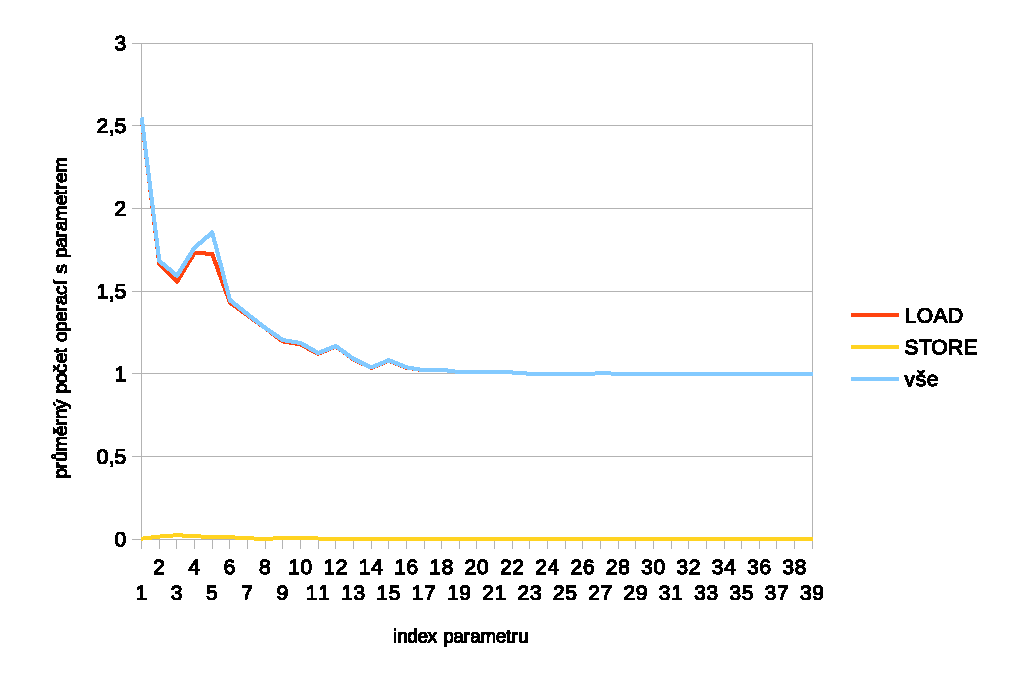
\includegraphics[scale=0.9]{fig/params}
\caption{Průměrné počty operací s parametry metod.}\label{params}
\end{figure}

\begin{figure}[h!]
\centering
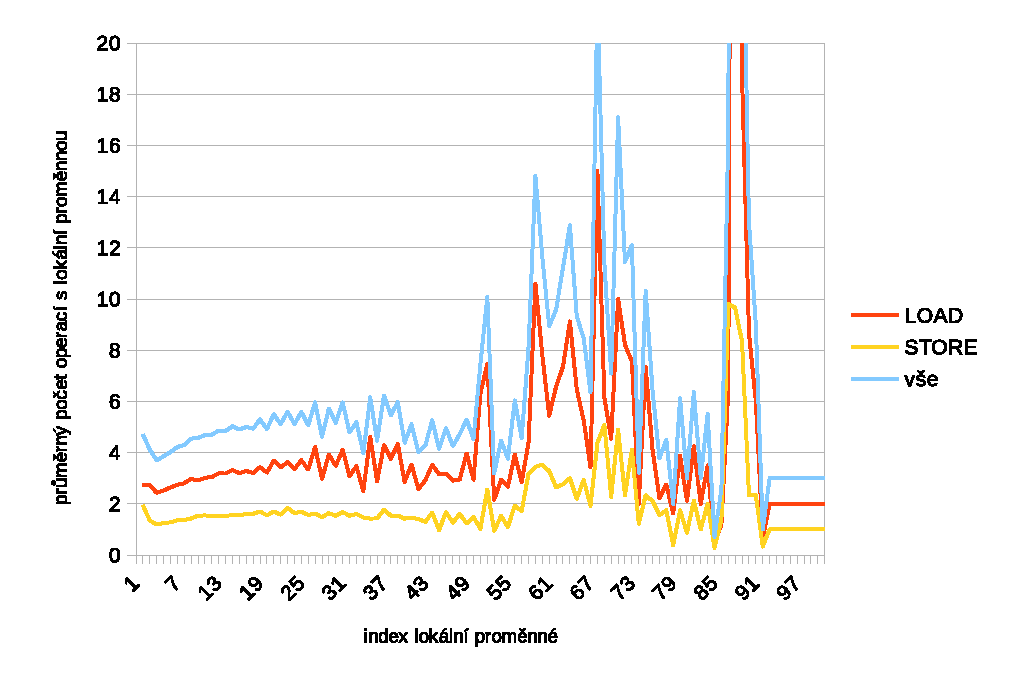
\includegraphics[scale=0.9]{fig/locals} 
\caption{Průměrné počty operací s lokálními proměnnými.}\label{vars}
\end{figure}

\section{Vyhodnocení}\label{AnalysisSummary}

%%%%%%%%%%%%%%%%%%%%%%%%%%%%%%%%%%%%%%%%%%%%%%%%%%%%%%%%%%%%%%%%%%%%%%%%%%
\chapter{Conclusion}


%=========================================================================


%=========================================================================
 % viz. content.tex

  % Pouzita literatura
  % ----------------------------------------------
\ifczech
  \bibliographystyle{czechiso}
\else 
  \bibliographystyle{plain}
%  \bibliographystyle{alpha}
\fi
  \begin{flushleft}
  \bibliography{literature} % viz. literature.bib
  \end{flushleft}
  \appendix
  
  \chapter{Obsah CD}

Přiložené CD obsahuje následující soubory:
\medskip

\begin{tabular} {l l}
\texttt{xponco00.pdf} & Písemná zpráva ve formátu PDF.\\
\texttt{dp-xponco00.tar.gz} & Zdrojové texty písemné zprávy.\\
\texttt{app-xponco00.tar.gz} & Zdrojové soubory aplikací s manuálem.\\
\texttt{data-xponco00.tar.gz} & Analyzovaný vzorek dat.\\
\texttt{application} & Spustitelné soubory aplikací.\\

\end{tabular}

%\begin{itemize*}
%\item písemnou zprávu ve formátu PDF,
%\item zdrojové texty písemné zprávy,
%\item zdrojové soubory programů,
%\item spustitelné soubory programů,
%\item manuál.
%\end{itemize*}

%\chapter{Manual}
%\chapter{Konfigrační soubor}
%\chapter{RelaxNG Schéma konfiguračního soboru}
%\chapter{Plakat}


 % viz. appendix.tex
\end{document}
